\chapter{Software Requirements Specification}

%------------------------- 3.1 ---------------------------

\section{Functional Requirements}

Functional requirements describe the core capabilities that the system must provide. These requirements are derived from initial discussions with Safe Media AI and define the expected behavior of the system from a user perspective.

\begin{table}[htbp]
\centering
\begin{tabular}{|p{5cm}|p{9cm}|}
\hline
\textbf{Requirement} & \textbf{Description} \\ \hline

\textbf{Automatic Detection of Sensitive Information} & 
The system shall automatically detect sensitive information in images, including faces and textual content. \\ \hline

\textbf{Image File Support} & 
The system shall support commonly used image formats such as PNG and JPEG. \\ \hline

\textbf{Manual Editing of Detection Results} & 
The system shall allow users to review, modify, and remove detected regions before redaction is applied. \\ \hline

\textbf{Multiple Redaction Methods} & 
The system shall support different redaction techniques such as blurring, pixelation, and masking. \\ \hline

\textbf{Redaction Execution} & 
The system shall apply selected redaction methods to user-defined or detected regions. \\ \hline

\textbf{Process Speed} &
The detection process should not be noticeably longer than Safe Media AI's detection system. \\ \hline

\textbf{System Integration Capability} & 
The system should be designed in a way that allows integration with external systems through well-defined interfaces. \\ \hline

\end{tabular}
\caption{Functional Requirements for the SafeVision System}
\label{tab:functional_requirements}
\end{table}

%------------------------- 3.2 ---------------------------

\section{Use Case Details}

The functional requirements are further illustrated through use cases, which describe how users interact with the system to achieve specific goals.

Figure~\ref{fig:safevision_usecase} presents a high-level overview of the system’s use cases.

\begin{figure}[htbp]
    \centering
    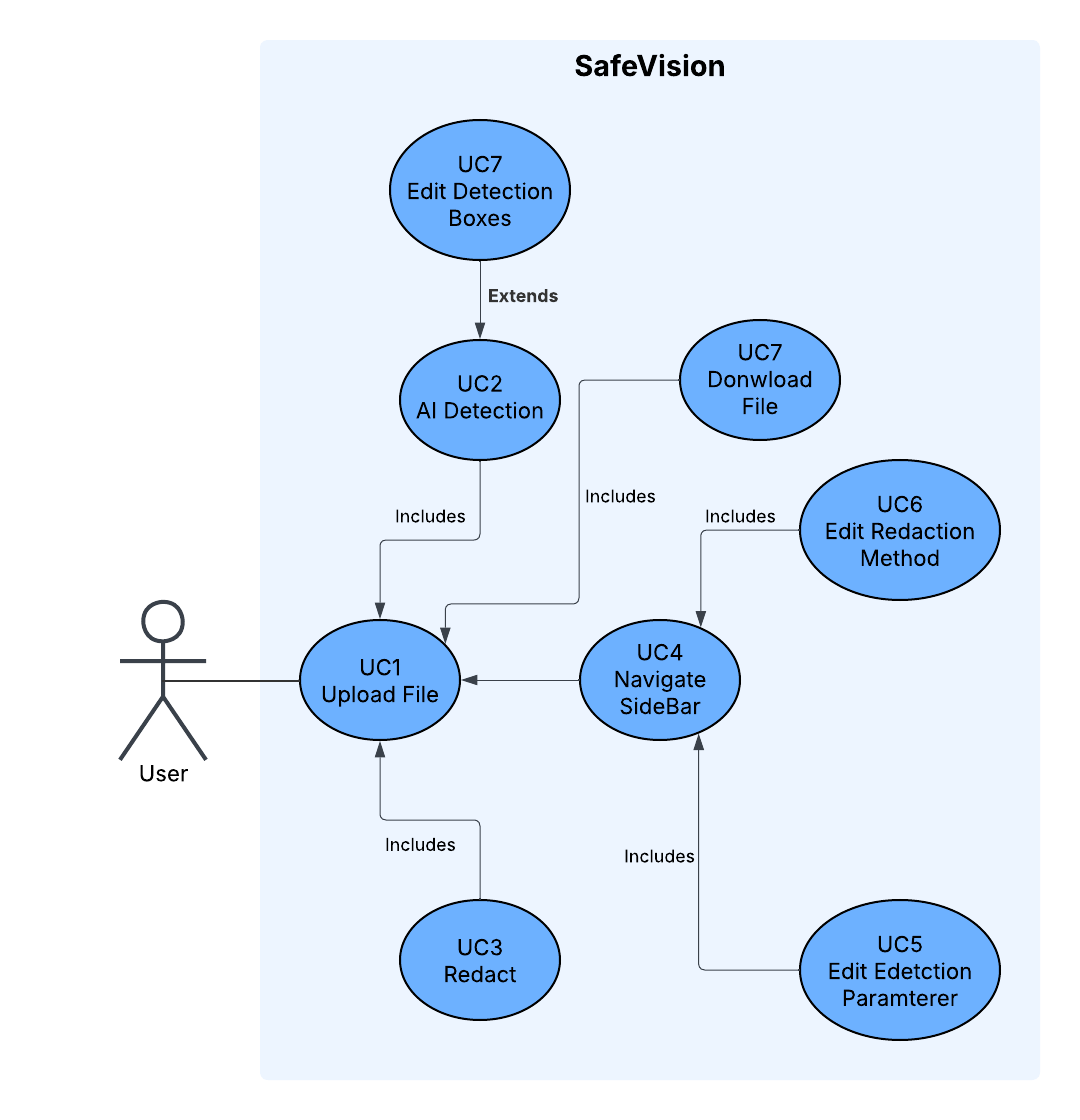
\includegraphics[width=0.8\textwidth]{figures/images/chapter-3/SafeVisionUseCase.png}
    \caption{Use case diagram for the SafeVision system}
    \label{fig:safevision_usecase}
\end{figure}

The primary workflow of the system consists of detecting sensitive information in images and applying redaction based on user input. These interactions are further detailed using sequence diagrams.

\subsection{Image Detection Scenario}

The detection process begins when a user uploads an image through the interface. The system analyzes the image and identifies regions that may contain sensitive information.

The detected regions are then presented to the user, allowing them to review and adjust the results before proceeding. This ensures that the user remains in control of the detection outcome.

\begin{figure}[htbp]
    \centering
    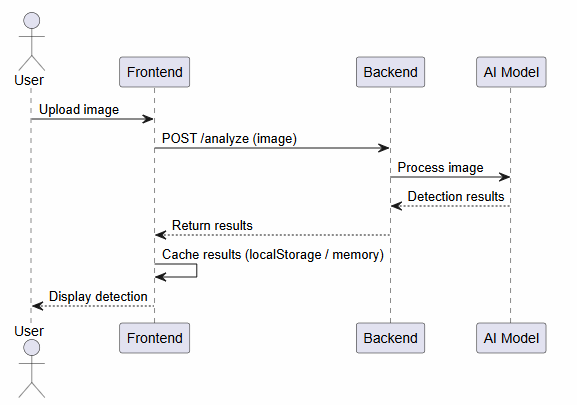
\includegraphics[width=0.9\textwidth]{figures/images/chapter-3/SequenceDetection.png}
    \caption{Sequence diagram illustrating the image detection interaction}
    \label{fig:sequence_detection}
\end{figure}

\subsection{Redaction Scenario}

After reviewing the detected regions, the user can modify the selected areas and choose a redaction method. The system then applies the redaction and generates a processed image.

The final result is presented to the user, allowing verification that sensitive information has been properly anonymized.

\begin{figure}[htbp]
    \centering
    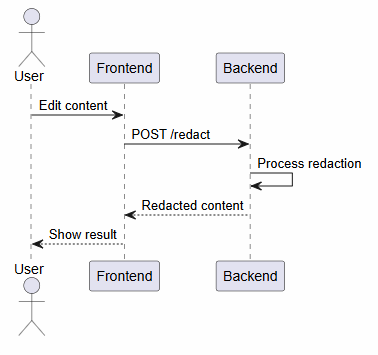
\includegraphics[width=0.9\textwidth]{figures/images/chapter-3/SequenceRedaction.png}
    \caption{Sequence diagram illustrating the redaction interaction}
    \label{fig:sequence_redaction}
\end{figure}

These scenarios demonstrate how the system combines automated processing with user control, ensuring both usability and reliability in handling sensitive information.

%------------------------- 3.3 ---------------------------

\section{Non-Functional Requirements}

Beyond the core functional capabilities of detecting and redacting sensitive information, the system must satisfy several non-functional requirements. These requirements define the overall quality attributes of the system and guide architectural and implementation decisions.

The non-functional requirements for this project are categorized into four main areas: \textit{security}, \textit{performance}, \textit{usability}, and \textit{maintainability}, as illustrated in Figure~\ref{fig:non_functional_req}.

\begin{figure}[htbp]
    \centering
    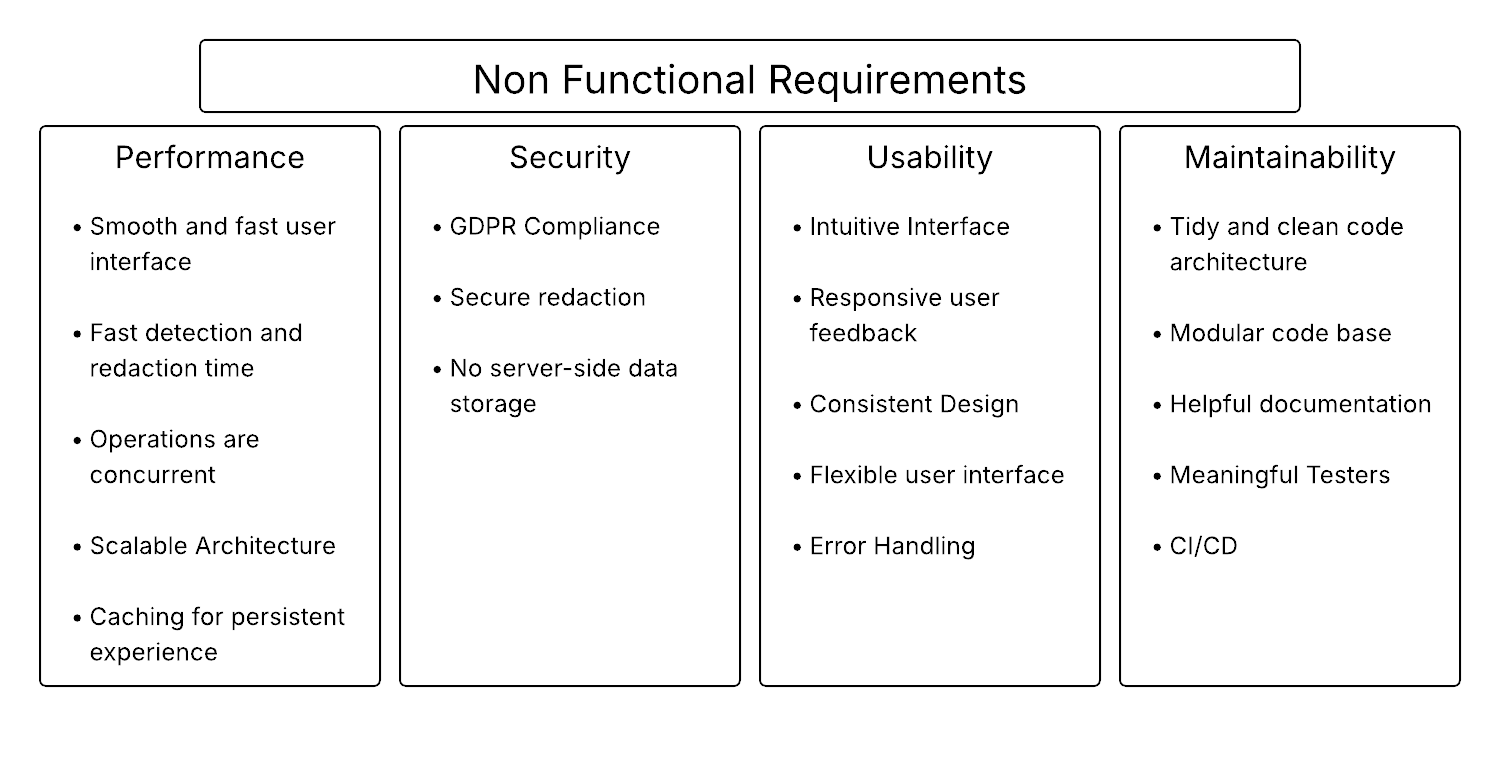
\includegraphics[width=0.8\textwidth]{figures/images/chapter-3/NonFunctionalReq.png}
    \caption{Overview of Non-Functional Requirements}
    \label{fig:non_functional_req}
\end{figure}

\subsubsection{Security}

Security requirements focus on ensuring that sensitive information is handled in a safe and compliant manner. The system is designed in accordance with GDPR, ensuring that personal data is processed responsibly and in line with regulatory standards.

Secure redaction is a central aspect of the system, meaning that sensitive information is properly anonymized before any output is presented to the user. This reduces the risk of exposing identifiable data.

Additionally, the system does not store any data on the server. All processing is performed temporarily, ensuring that sensitive images are not persistently stored. This minimizes potential risks related to data breaches and unauthorized access.

\subsubsection{Performance}

Performance requirements ensure that the system operates efficiently and provides a smooth user experience. The user interface is designed to be responsive and fast, allowing users to interact with the system without delays.

Fast detection and redaction time is essential to reduce waiting time when processing images. The system is optimized to perform these operations efficiently.

The system supports concurrent operations, enabling multiple processes or users to interact with the system simultaneously without significant performance degradation.

A scalable architecture is implemented to handle increasing workloads and larger datasets if needed. Additionally, caching mechanisms are used to provide a more persistent and efficient user experience by reducing unnecessary repeated computations.

\subsubsection{Usability}

Usability requirements focus on making the system intuitive and easy to use. The interface is designed to be simple and understandable, allowing users to quickly learn how to interact with the system.

Responsive user feedback ensures that users receive immediate visual or system responses when performing actions. This helps users understand the system state and results of their interactions.

A consistent design is maintained across the application, making navigation predictable and reducing user confusion. The interface is also flexible, allowing it to adapt to different user needs and workflows.

Error handling is implemented to guide users when issues occur. Clear and informative messages help users recover from errors and continue their tasks efficiently.

\subsubsection{Maintainability}

Maintainability requirements ensure that the system can be easily developed, updated, and extended over time. The system follows a tidy and clean code architecture, making it easier to understand and maintain.

A modular code base is used to separate different components of the system. This allows developers to modify or extend parts of the system without affecting the entire application.

Helpful documentation is maintained to support development and onboarding of new contributors. This ensures that the system remains understandable throughout its lifecycle.

Testing plays an important role in maintainability. Meaningful tests are implemented to verify system functionality and ensure stability during future changes.

Finally, CI/CD practices are used to support continuous integration and deployment, enabling efficient development workflows and reliable system updates.

%------------------------- 3.4 ---------------------------

\section{Requirement Prioritization}

To guide development and ensure that critical functionality was implemented first, the requirements were prioritized based on their importance, impact on the system, and input from Safe Media AI.

The prioritization reflects a practical development approach, where essential functionality was implemented first, followed by desirable features, while less critical functionality was considered for potential future work.

\begin{itemize}
    \item \textbf{High Priority:}
    \begin{itemize}
        \item Automatic detection of sensitive information
        \item Manual editing capabilities
        \item Redaction functionality
        \item Image format support (PNG/JPEG)
    \end{itemize}

    \item \textbf{Medium Priority:}
    \begin{itemize}
        \item Multiple redaction methods
        \item Fast processing performance
        \item Video capabilities
    \end{itemize} 

    \item \textbf{Lower Priority:}
    \begin{itemize}
        \item Recognition capabilities
        \item Advanced filtering and customization options
        \item Complex user preference options
        \item Metadata extraction and flexibility
    \end{itemize}
\end{itemize}

This prioritization ensured that the most important system features were developed within the project timeframe while still allowing flexibility for future extensions and improvements.